\documentclass[twoside]{report}
\usepackage[utf8]{inputenc}
%\usepackage[english]{babel}
\usepackage{amsthm}
\usepackage{tkz-fct} 
\usepackage{thmtools}
\usepackage[margin=1in]{geometry}
\usepackage{amsmath,amssymb}
\usepackage{multicol}
\usepackage{graphicx}
\usepackage{tikz}
\usepackage{listings}
\usetikzlibrary{positioning} 
\usetikzlibrary{calc,patterns,angles,quotes}
\usetikzlibrary{calc,arrows, arrows.meta}
\tikzset{
  arrow/.pic={\path[tips,every arrow/.try,->,>=#1] (0,0) -- +(.1pt,0);},
  pics/arrow/.default={triangle 90}
}
\usepackage{pgfplots}% also loads graphicx
\pgfplotsset{compat=1.11} %width=10cm,
\usetikzlibrary{backgrounds}
\usepackage{siunitx}
\sisetup{per-mode=fraction} %,fraction-function = \nicefrac}
\DeclareSIUnit{\gallon}{gal}
\usepackage{fancyhdr}
\usepackage{pst-node}
\psset{nodesep=2pt,linearc=2pt,arrows=->,linecolor=blue,arrowinset=0}
\def\lbl#1{\ncput*{\text{\tiny #1}}}
\usepackage{xcolor}
\usepackage{tcolorbox}
\usepackage{lmodern}
\usepackage{relsize}
\newcommand{\highlight}[1]{%
  \colorbox{red!50}{$\displaystyle#1$}}
\usepackage{url}
\usepackage{cancel}
\usepackage{float}
\usepackage[numbers]{natbib}
\usepackage{setspace}
\usepackage{subcaption}
\usepackage{varwidth}
% set the arrows as stealth fighters (personal preference)
\tikzset{>=stealth}
\captionsetup[figure]{labelfont={bf},name={Figure},labelsep=period}

\declaretheoremstyle[
  spaceabove=6pt, spacebelow=6pt,
  headfont={\color{blue}\fontfamily{cmss}\selectfont\bfseries},
  notefont=\fontfamily{cmss}\selectfont\bfseries, notebraces={(}{)},
bodyfont=\fontfamily{cmss}\selectfont\itshape,
  postheadspace=1em,
]{mystyle}
\declaretheorem[style=mystyle,numbered=no]{definition}
\declaretheorem[style=mystyle,numbered=no]{lemma}

\declaretheoremstyle[
  spaceabove=6pt, spacebelow=6pt,
  headfont={\color{black} \fontfamily{cmss}\selectfont\bfseries},
  notefont=\fontfamily{cmss}\selectfont\bfseries, notebraces={(}{)},
bodyfont=\fontfamily{cmss}\selectfont,
  postheadspace=1em,
  qed=$\triangle$
]{mystyle2}
\declaretheorem[style=mystyle2,numbered=no]{remark}

\declaretheoremstyle[
  spaceabove=6pt, spacebelow=6pt,
  headfont={\color{orange} \fontfamily{cmss}\selectfont\bfseries},
  notefont=\fontfamily{cmss}\selectfont\bfseries, notebraces={(}{)},
bodyfont=\fontfamily{cmss}\selectfont,
  postheadspace=1em,
  qed=$\triangle$
]{mystyle3}
\declaretheorem[style=mystyle3,numbered=no]{example}

\declaretheoremstyle[
  spaceabove=6pt, spacebelow=6pt,
  headfont={\color{blue} \fontfamily{cmss}\selectfont\bfseries},
  notefont=\fontfamily{cmss}\selectfont\bfseries, notebraces={(}{)},
  bodyfont=\fontfamily{cmss}\selectfont\itshape,
  postheadspace=1em,
  qed=
]{mystyle4}
\declaretheorem[style=mystyle4,numbered=no]{law}

\declaretheoremstyle[
  spaceabove=6pt, spacebelow=6pt,
  headfont={\color{blue} \fontfamily{cmss}\selectfont\bfseries},
  notefont=\fontfamily{cmss}\selectfont\bfseries, notebraces={(}{)},
bodyfont=\fontfamily{cmss}\selectfont,
  postheadspace=1em,
  qed=
]{mystyle5}
\declaretheorem[style=mystyle5,numbered=no]{strategy}

\declaretheoremstyle[
  spaceabove=6pt, spacebelow=6pt,
  headfont={\color{blue} \fontfamily{cmss}\selectfont\bfseries},
  notefont=\fontfamily{cmss}\selectfont\bfseries, notebraces={(}{)},
bodyfont=\fontfamily{cmss}\selectfont\itshape,
  postheadspace=1em,
  qed=
]{mystyle6}
\declaretheorem[style=mystyle6,numbered=no]{theorem}


\renewcommand{\qedsymbol}{\rule{0.7em}{0.7em}}
\renewenvironment{proof}{{\bfseries \fontfamily{cmss} \scshape Proof:}}



\newcommand{\reporttitle}{###}
\newcommand{\reportauthor}{Kai Cooper\\Yacine Trad}
\newcommand{\reportsecondauthor}{}
\newcommand{\reportthirdauthor}{}
\newcommand{\reportfourthauthor}{}
\newcommand{\reportfifthauthor}{}
\newcommand{\supervisor}{Dr. Medhi Ghoulam}

\date{June 2021}

\renewcommand{\chaptername}{Part}
\newcommand{\lap}{\nabla^2}
\newcommand{\dif}[1]{\text{d}#1}

\newcommand{\code}{\texttt}

\definecolor{fcolor}{RGB}{0,255,255}


\begin{document}
\begin{spacing}{1}
% Last modification: 2015-08-17 (Marc Deisenroth)
\begin{titlepage}

\newcommand{\HRule}{\rule{\linewidth}{0.5mm}} % Defines a new command for the horizontal lines, change thickness here


%----------------------------------------------------------------------------------------
%	LOGO SECTION
%----------------------------------------------------------------------------------------

%\includegraphics[width = 4cm]{}\\[0.5cm] 

\center % Center remainder of the page

%----------------------------------------------------------------------------------------
%	HEADING SECTIONS
%----------------------------------------------------------------------------------------

\textsc{\Large École Polytéchnique Fédérale de Lausanne}\\[0.5cm] 
\textsc{\large Department of Mathematics}\\[0.5cm] 

%----------------------------------------------------------------------------------------
%	TITLE SECTION
%----------------------------------------------------------------------------------------

\HRule \\[0.4cm]
{ \huge \bfseries \reporttitle}\\ % Title of your document
\HRule \\[1.5cm]
 
%----------------------------------------------------------------------------------------
%	AUTHOR SECTION
%----------------------------------------------------------------------------------------

\begin{minipage}{0.4\textwidth}
\begin{flushleft} \large
\emph{Authors:}\\
\reportauthor\\ % Your name
\reportsecondauthor\\
\reportthirdauthor\\
\reportfourthauthor\\
\reportfifthauthor
\end{flushleft}
\end{minipage}
~
\begin{minipage}{0.4\textwidth}
\begin{flushright} \large
\emph{Supervisor:} \\
\supervisor % Supervisor's Name
\end{flushright}
\end{minipage}\\[4cm]


%----------------------------------------------------------------------------------------
%	FOOTER & DATE SECTION
%----------------------------------------------------------------------------------------
\vfill % Fill the rest of the page with whitespace

\makeatletter
\@date
\makeatother


\end{titlepage}
\fontfamily{cmss}\selectfont
\tableofcontents



\begin{abstract}

\end{abstract}


\chapter{Discovery and Assessment of optimal cryptocurrency trading strategies} 
\section{Introduction}

\begin{itemize}
    \item 
The goal of this project is to proceed to the analysis of an optimal trading (buy-and-sell) strategy for the market of Cryptocurrencies. We expect such a strategy, if sucessful, also applicable to the case of traditionnal stock markets. (note: Cryptocurrencies data are traditionnaly more easily and freely available than stock markets data, which are often pricey)
    \item
The first part of the project will consist in showing you how to access the data of all historical data available on Binance. We choose Binance because it is one, if not the only exchange, with a properly working API which also have historical data up to 2017 and for the widest range of cryptocurrency pairs, and therefore the most diverse range of applicable trading strategy (arbitrage, sentiment-driven prices, trends, market making, etc).
    \item{
If you don't want to get your hands dirty (which is understandable) navigating through the code to download the data, simply download a set of the date at this link : \url{https://drive.switch.ch/index.php/s/URDxQbEv8LqSkB2}}

\end{itemize}



\section{Data Extraction}

\begin{itemize}
\item{To extract the Data, you can do so as per the call of getuptodate\_binance\_data.update\_data\_for\_basepair(base\_pair=\'USDT\', nb\_symbols\_limit=5, bin\_size=\'1d\') in get\_ohlc\_historical\_data.ipynb}

\item{The data will be saved in a folder named Binance\_OHLC\textquotesingle located within a 'Data' folder within your project folder. If you do not have such folders, create some. (If you are familiar with \'chdir\' python function to change and work with your choice directory you can ignore this remark).}

\item{The code in get\_uptodate\_binance\_data.py contains a global variable 'main_directory' which has the name of my project folder I am working on. I recommend you call your project folders with the same name.}
\end{itemize}


\section{Data Cleaning}

\begin{itemize}
    \item 
We use the clean\_csv() function to clean the newly doownloaded data file. In particular, we setup timestamp in datetime format, to allow us to have an easier handling of the data later on.
    \item
We also select a subset of the columns of interest to us. In particular we keep keep the following columns: ['timestamp', 'open', 'high', 'low', 'close', 'volume', 'time_diff_in_days', 'time_diff_in_min'].
    \item
Note that we have never encountered any NA values or other seemingly out-of-place values that would need to be rejected. Indeed, so called 'out-of-place values' or any other outliers kind of value are strong indicators which require further investigations and may be relevant to dedicated algorithmic trading strategies. We absolutely do not want to remove them as we may be tempted to do in some other contexts in data science.
    \item
Discrepencies in the timestamp of our data : Missing time periods. Every once in a while there is a major crash in cryptocurrencies market (i.e. prices dropping significantly). This leads to a massive amount of people trying to connect to the cryptocurrencies exchange platforms to try to sell (or buy) some cryptocurrencies.This often results in the exchange becoming unavailable, their server not being able to handle so many connections attempts at once. This explains the missing data in historical cryptocurrencies prices data (It can be for a couple of minutes up to a couple of hours). We therefore compute 'time_diff_in_days' and 'time_diff_in_min' to spot any such discrepancies in the timestamp.
    \item
You can find the code in the get_uptodate_binance_data.py file

\end{itemize}


\section{Multiple Datasets Analysis
}

\begin{itemize}
    \item 
Once an analysis is performed on a dedicated dataset (e.g. 1 hour BTC/USDT historical data), the same statistical analysis can be performed over any dataset (e.g. 1 minute ETH/CHF historical data), since the data structure (i.e. the columns, open, high, low, close) is the same. We will do so later on in the project.
    \item
We downloaded the data for hundreds of cryptocurrency pairs over various timeframe (1 day, 1 hour, 1 minute, etc) so that we can perform meta-analysis and/or repeat the small single-pair dataset analysis over all other sets

\end{itemize}


\section{Exploratory Data Analysis}
In this section, we present some exploratory data analysis for our dataset.

\begin{figure}[!htbp]
    \centering
    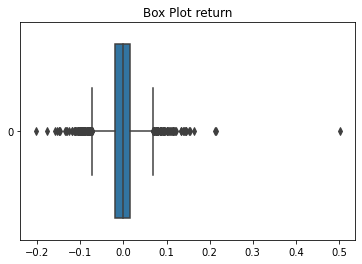
\includegraphics[scale = 0.5]{Images/Box Plot of Return.png}
    \caption{Box plot of log-return}
    \label{log return box}
\end{figure}

Figure \ref{log return box} shows the box plot of log-return of BTC. As can be seen from the graph, there are many outliers of the box plot. So it is reasonable to say that the distribution of log-return is not a normal distribution. More evidence will be given in the following sections.

\begin{figure}[!htbp]
    \centering
    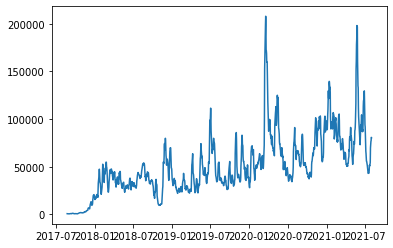
\includegraphics[scale = 0.5]{Images/Volume Rolling Average.png}
    \caption{7 day rolling average of the volume}
    \label{7day rolling volume}
\end{figure}

Figure \ref{7day rolling volume} is about 7 days rolling average of the volume. From this figure, we see that the volume oscillate during our examining period. The volume sometime change drastically for a certain day. However, with the existence of up and down signals, we see there is a trend of volume increasing from the beginning of 2017-07 to 2021-07.






\section{key concepts}

The goal of this project is to proceed to the analysis of an optimal trading (buy-and-sell) strategy for the market of Cryptocurrencies. Our analysis will be made on cryptocurrency pairs.\\
These pairs allow us to compare costs between different cryptocurrencies. They are helpful for illustrating the relative worth of coins. For example,the question how much Bitcoin (BTC) equals in Ethereum (ETH) will be answered by the value of the pair BTC/ETH.
In this report we are dealing with the BTC/USDT pair. USDT stands for Tether which is a stable coin in which each token is backed by a U.S Dollar.\\
The price of a token depends on the market cap of the currency and how many tokens are issued. And since there are hundreds of cryptocurrencies dealing with their prices can become very cumbersome and lack clarity. For that very reason, we have chosen to deal in our analysis with log-returns.
Indeed, the price of a currency is not what is of interest to us but rather it's evolution. By studying prices we would be confronted with values that don't have an intrinsic meaning, However with log returns we will have an idea of the evolution in percentages, which is way more useful. To sum it up, this allows measuring a lot of variables in a comparable metric, thus enabling evaluation of analytic relationships amongst two or more variables despite originating from price series of unequal values. \\
Concretely, if we are doing our study on a currency at time $i$ which is valued at price $p_i$. The log-return for the period $t$ is:
$$\log(\frac{p_i}{p_{i-t}})$$\\

Another important property is the additivity of the log-return. If our price at $t_1$ is $p_1$, it changes to $p_2$ at $t_2$ and move to $p_3$ at $t_3$. The log return from $t_1 $ to $t_2$ is $\log (p_2) - \log (p_1)$, the log return from $t_2 $ to $t_3$ is $\log (p_3) - \log (p_2)$. Therefore, it is clear that the log return from $t_1 $ to $t_3$ is $\log (p_3) - \log (p_1)$. This can be calculated easily. However, if we use simple return, the return should be $\frac{p_3}{p_1}$ instead of $\frac{p_3}{p_2} + \frac{p_2}{p_1}$. Hence, log-return is easier to apply in the real world.




 An interesting observation one can make when plotting the log-returns is that they are supposed to be normally distributed, however when looking at Figure 1.1 we can see that the mean is slightly tilted to the positive side which indicates that BTC has been a good investment overall.
 

\section{Analysis of extremes}

In financially related fields, the question of extreme values is indubitably an important one. For example: stock market crashes, interest rates  insurance pricing based on life expectancy are all fields in which it would be necessary to consider the very unlikely, atypical events. The analysis of cryptocurrency trajectories is no different, indeed, it would certainly be of interest to a trader to be aware at what rate the cryptocurrency market experiences sudden but large deviations from its present state. Recently, in fact, in March of $2020$, Bitcoin crashed. In the midst of the COVID-19 outbreak, the price of Bitcoin fell dramatically, see Figure \ref{fig:logreturn_17_21} for a visualisation.



In light of this, it is not unnatural to ask the corresponding statistical question in the context of extremes. In Figure \ref{fig:hist_logreturn_17_21}, we can see that the distribution of log returns for our data set admits very heavy tails. Admittedly, one is aware of the very large anomaly which greatly negatively skews the data in a noticeable fashion. However, in spite of this, using a common statistical rule for eliminating outliers based upon the quartiles of a distribution, we find, as in Figure \ref{fig:distplots_sans_outliers}, the data still exhibits this skewed behaviour. This sparks interest in using extreme value theory to aid our understanding of it.\\

Let $(X_i)_{i=1}^n$ be a random sample from some distribution $F$, and $M_n = \max(X_1, \ldots, X_n)$ be the $n$th order statistic. If there exist sequences $(a_n) \subset \mathbb{R}^+$ and $(b_n) \subset \mathbb{R}$ such that $(M_n - b_n)/a_n \overset{D}{\to} G$, for some distribution $G$, then $G$ must be of extremal value type, that is, \[
G(x; \eta, \tau, \xi) = \begin{cases}
\exp\left[-\left\{1+\xi(x-\eta)/\tau\right\}_+\right], & \xi \ne 0\\
\exp\left[-\exp\left\{-(x-\eta)/\tau\right\}\right], & \xi = 0
\end{cases}
\]
where $\eta, \tau$ and $\xi$ are location, shape and scale parameters respectively. \begin{remark}
Extreme value theory does not apply singly to maxima, if $M_n' = \min(X_1, \ldots, X_n)$, then we have that $M_n' = -\max(-X_1, \ldots, -X_n)$ and so the corresponding limiting distribution function is $1-G(-x)$. 
\end{remark}

Studying maxima in this way is known as the \textbf{block maxima approach}, since one groups data and considers fitting the distribution to the maxima across all groups, for example: annual global extreme temperatures. There is another approach, called \textbf{peaks over thresholds}, which studies the exceedance of a random sample beyond a predefined threshold. This will be discussed later.


The goal now, therefore, is to fit this model to our data, i.e. by finding the unknown parameters. To this end, we use the $\code{R}$ package $\code{evd}$ which gives useful functions for extremal modelling and makes plotting diagnostics straightforward. The function $\code{fgev}$ fits the block maxima (or minima when appropriately transformed) to the model through maximum likelihood estimation. Assuming certain regularity conditions, we can derive estimates and corresponding uncertainties from our method.  
\begin{figure}
    \centering
    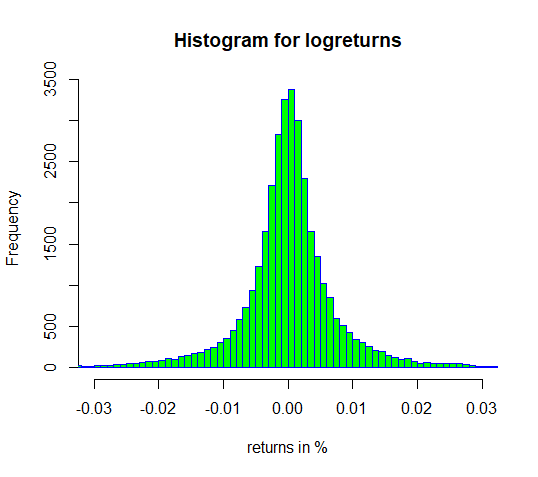
\includegraphics[width=\linewidth, height=3.5in]{TestPlots/Histogram log-returns2.png}
    \caption{Distribution of log returns using data from August 2017 to August 2021. The distribution shows some quite heavy tails.}
    \label{fig:hist_logreturn_17_21}
\end{figure}

\begin{figure}
    \centering
    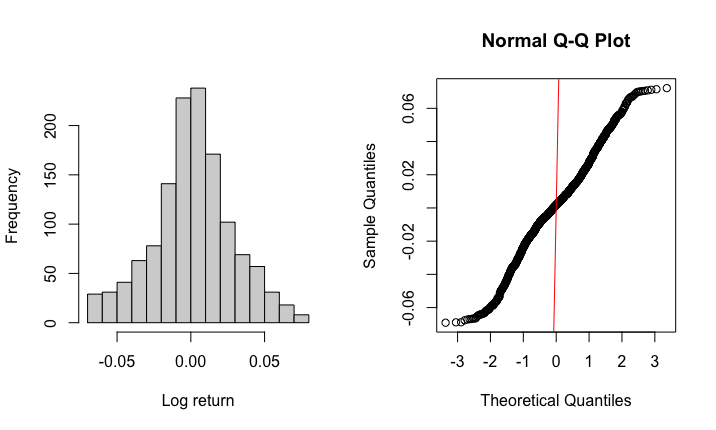
\includegraphics[width=\linewidth]{Extremal Modelling/distplots_sans_outliers.png}
    \caption{Distribution of log returns having eliminated outliers and a QQ plot of the data against a standard normal random variable. Clearly the data is still heavily tailed.}
    \label{fig:distplots_sans_outliers}
\end{figure}










\end{spacing}
\end{document}
